\chapter{Research results}

In this chapter the research results are discussed.
\todo{create better introduction}
For each research question, a separate section is used. 

\section{How can the new Analysis Website be set up outside of \testar? (\ref{rq:application-outside-testar})} \label{sec:components-explained}
The new application is written outside the \testar application. Doing so makes it possible to work without the context and dependencies of \testar and allows the application to be written in a language more known by the developer. The only dependency it has with \testar is the OrientDB graph database.

Besides OrientDB, the solution is divided into two major parts. A \testar proxy, named .NET server, and a new \testar analysis website. As the name suggests, they are built and created in Framework from Microsoft: .NET Core (version 6) \footnote{\url{https://dot.net}}. .NET is an open-source, cross-platform framework. An application created with .NET will run on Windows, Linux and macOS. 

\begingroup
\captionsetup{type=figure}
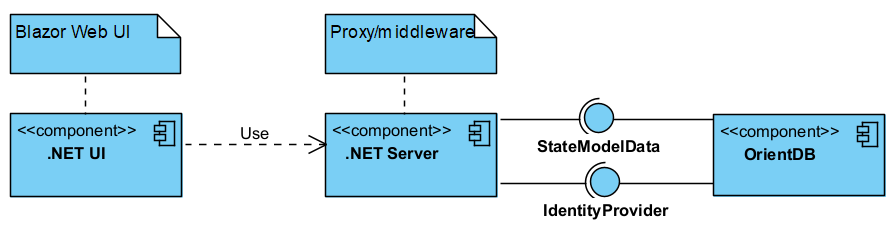
\includegraphics[scale=0.7]{images/server-ui-comp.png}
\captionof{figure}{.NET UI - Server and OrientDb component model (UML 2.0)}\label{fig:components}
\endgroup

Figure \ref{fig:components} shows the three components making up the system. The state model data that \testar generated is saved into the OrientDB graph database, and the .NET server uses the same database. The new \testar analysis website connects to the .NET server. In the following sections, the different components are explained. 

Since both the .NET server and the website are running .NET, they use the same core library. Using the same core library makes it easy to share code. As an extra benefit, the core library can be reused in other applications dedicated to a single task. 

\subsection{OrientDB Component}
OrientDB is the data storage for \testar. The new application presents the data to the user. In order to query the data, the \verb|REST| API of OrientDB is used. A \verb|POST| is sent to OrientDB with the query and parameters in the request's body. An example of the body is displayed in listing \ref{code:example-body}.

\begin{lstlisting}[language=xml, caption=Get AbstractStateModel by the model identifier, label=code:example-body]
{
  "command": "SELECT FROM AbstractStateModel WHERE modelIdentifier = :id",
  "parameters": {
    "id": "1chdi5230521708089"
  }
}
\end{lstlisting}

An alternative way of querying the data is using the query \verb|GET| operation. While it is easy to query the data, it is vulnerable to SQL injection since the parameters are directly used in the SQL query. Those parameters can be changed by user input. 

The current solution in which the queries are sent from the UI to the .NET server is not entirely foolproof either. For example, using the Burp Suite is still possible to alter the \verb|POST| message body and attack the OrientDB database. This issue can be circumvented by setting up \verb|REST| endpoints on the.NET Server that created the SQL calls on the server-side.

It is not recommended to expose the OrientDB database directly to a public network \cite{orientdb-security}. Besides the orientDb recommended best practices and issues accessing the database on a web frontend, a proxy/middleware component is built. The following section explains the .NET server in more detail. 

\subsection{.NET Server} \label{sec:net-server}
The .NET Server serves as a proxy between the new \testar analysis website and the existing OrientDB graph database. It also provides an easy to use endpoint for other to-be-build applications.

The need for the .NET Server was due to browser restrictions and limitations in accessing the database. Two issues arose when the UI was trying to connect to the database. The issue was \acrfull{cors}. CORS is a security feature in which a web server can permit or deny requests from a website if the request was not made from a trusted source \cite{cors}. By default OrientDB does not permit other websites to use their \verb|REST| endpoints \cite{orientdb-webserver}. It is possible to enable CORS in the OrientDB configuration, but before the .NET application can be used, administrators should edit the OrientDB configuration. Although it would solve the CORS issue, a second issue involving the cookie is not solved.

The second issue prevented the analysis website from accessing and reading the cookie created by OrientDB. OrientDB saves a cookie, the session token. Before a user can query the data, it needs to sign in to OrientDB. Sign in is accomplished by executing a \verb|GET| command to the \verb|/connect/database| endpoint and providing the username and password, encoded with the base64 algorithm, as an authentication header. The OrientDB will return a \verb|200 OK| response with a \verb|osessionid| in the response headers if the credentials are valid. The \verb|osessionid| authenticates the user on future calls.

It was impossible to retrieve the \verb|osessionid| header and reuse it in the further data retrieval calls. Because the web browser blocked the session header, we could store the users' credentials in local storage, making them available for retrieval with a Cross-Site Scripting attack. Section \ref{sec:auth} will look into authentication and authorisation in more detail.

The OrienDB URL and name of the \testar state model database are provided in the server configuration. Based on user feedback, it is also possible to enable muti-database features. Enabling the multi-database feature enables to user to specify the name of the database during logging in. For example, if the user wants to connect to the database \verb|TestarData| and the username is \verb|Kirk|, the username for sign in becomes: \verb|TestarData\Kirk|.

\subsection{New \testar analysis website}
With the \testar application, it is possible to open an analysis website \cite{thesisMulders}. This website provided several features like viewing the available state models, Test sequences and a graph engine created with Cytoscape.js. The user has to install \testar on their machine to view this analysis website. This thesis presents a new website that can be used outside the \testar application. It got a fresh look and feel, created with Bootstrap\footnote{\url{https://getbootstrap.com}} and a noticeable increase in performance. Figure \ref{fig:ui-home-page} show the renewed available models screen. 

\newpage
\begingroup
\captionsetup{type=figure}
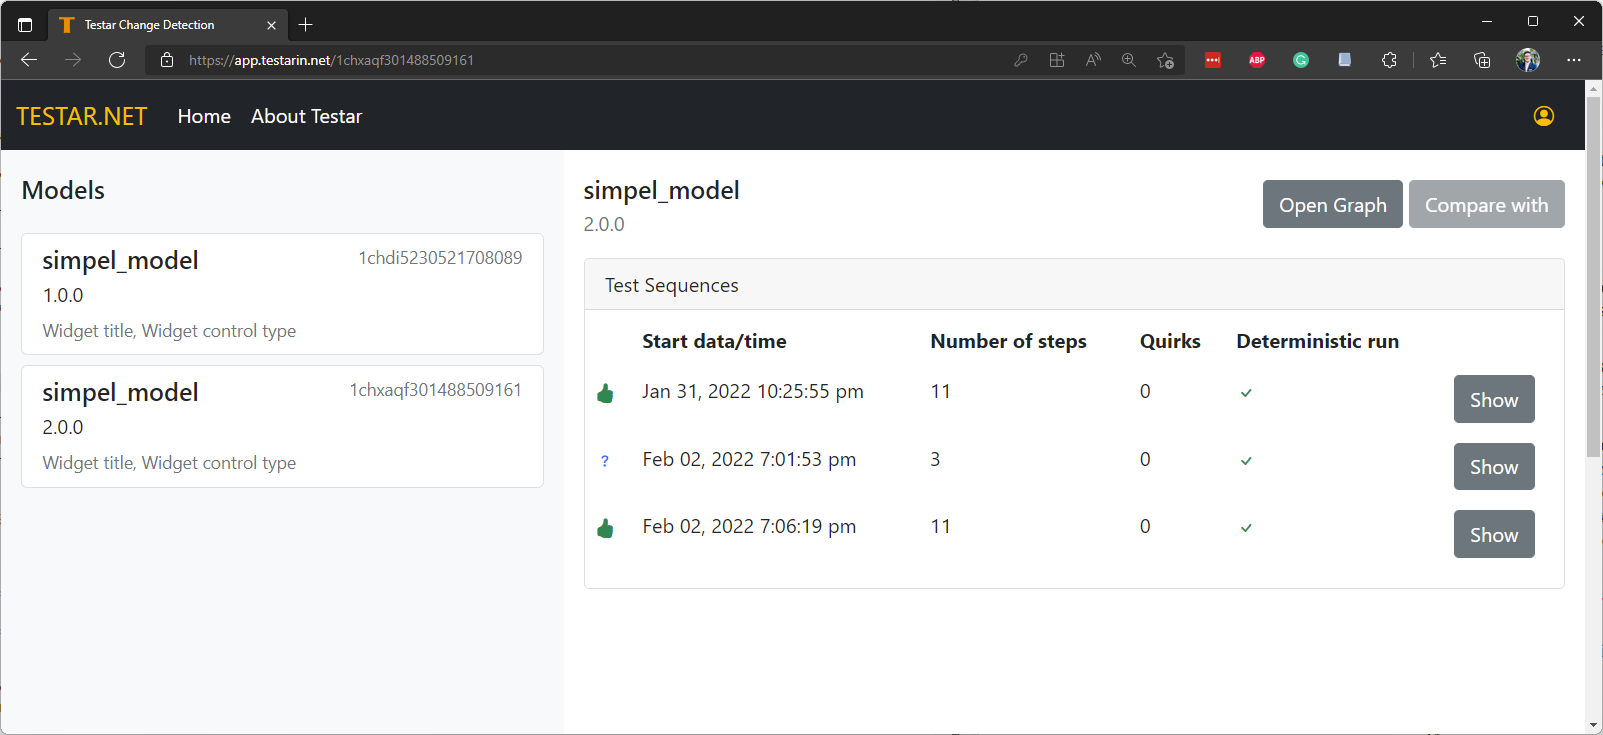
\includegraphics[scale=0.4]{images/ui-home-page.png}
\captionof{figure}{Available models in the new \testar website}\label{fig:ui-home-page}
\endgroup

The new \testar analysis website is created in Blazor. Blazor is an interactive web UI technology that allows running .NET code in the browser \cite{what-is-blazor}. For the graphical layer, Blazor uses HTML. Although some parts are still coded in Javascript, the application code is written in C\#. 

The code required to display the state graph, as shown in figure \ref{fig:graph-page}, has been copied from the original \testar source code. Besides the HTML layer and the retrieval of the raw model data, nothing has been altered. The graph engine is still using the Cytoscape.js library. 

\newpage
\begingroup
\captionsetup{type=figure}
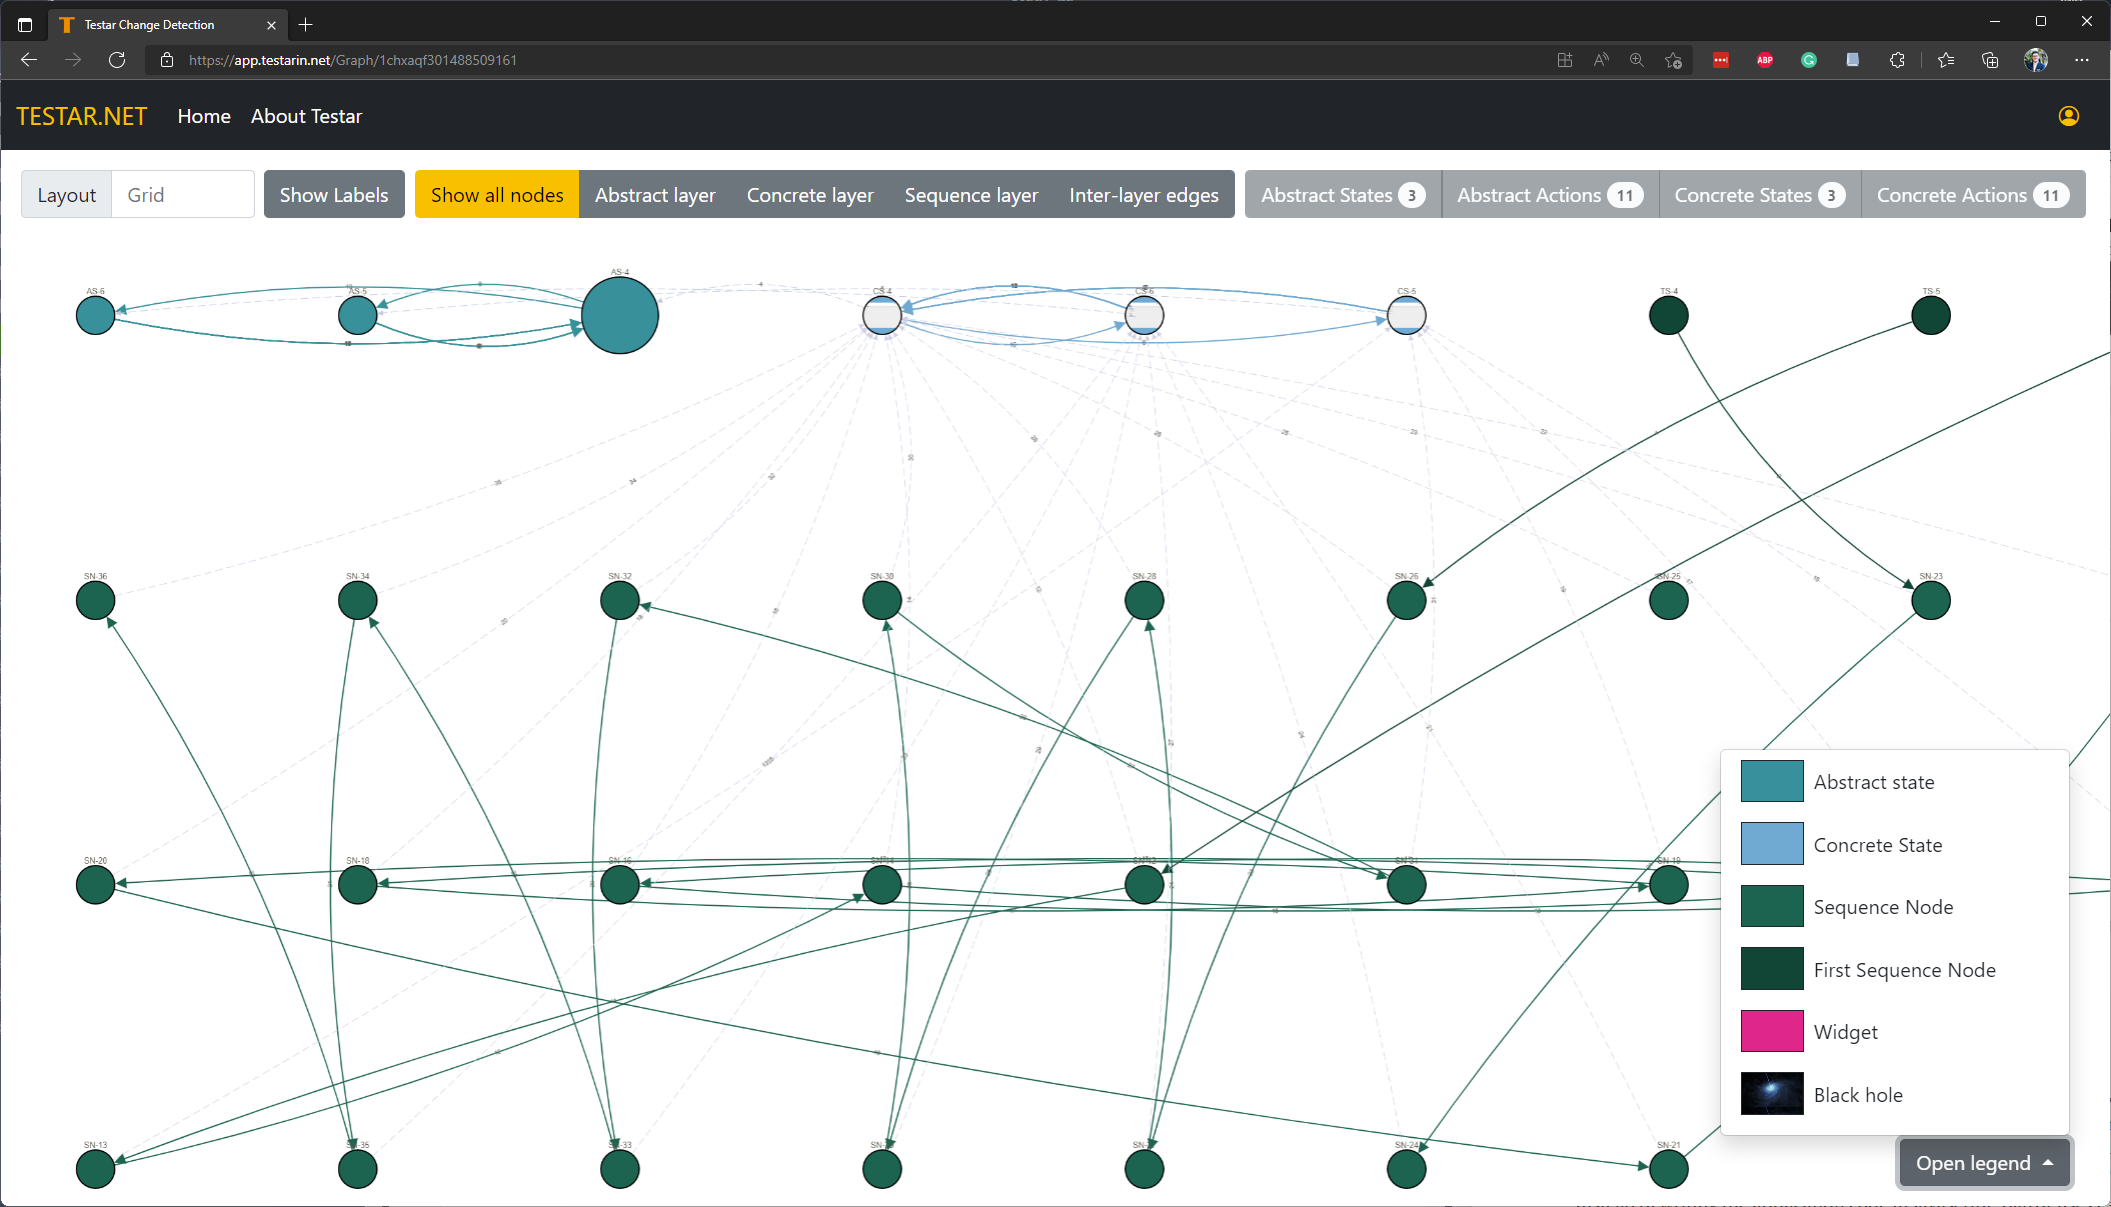
\includegraphics[scale=0.3]{images/graph-page.png}
\captionof{figure}{The new Graph page}\label{fig:graph-page}
\endgroup

\subsection{Authentication \& Authorisation} \label{sec:auth}
The .NET server helps with solving the security issues mentioned in ref{sec:net-server}  while still providing a secure and open authentication endpoint. External applications that want to use the endpoints must first authenticate with the .NET server upon it will return a \acrfull{jwt}. A JWT is a \textit{"compact, URL-safe means of representing claims to be transferred between two parties."} \cite{jones2015json}.

Before the user can use the \testar analysis website, it must authenticate itself. Figure \ref{fig:auth-sd} shows the sequence diagram of how the authentication flow is handled. Since the user identities are stored in the identity provider of the graph database, it is essential to note that the .NET server does neither handle authentication nor authorisation. The OrientDB Server handles the authentication and authorisation. The figure shows that the .NET server proxies the credentials and returns a JWT with the \verb|osessionid| as data. When the user provides incorrect credentials, the OrientDB will return a \verb|401 Unauthorised|, and the .NET server will return that status code.

\begingroup
\captionsetup{type=figure}
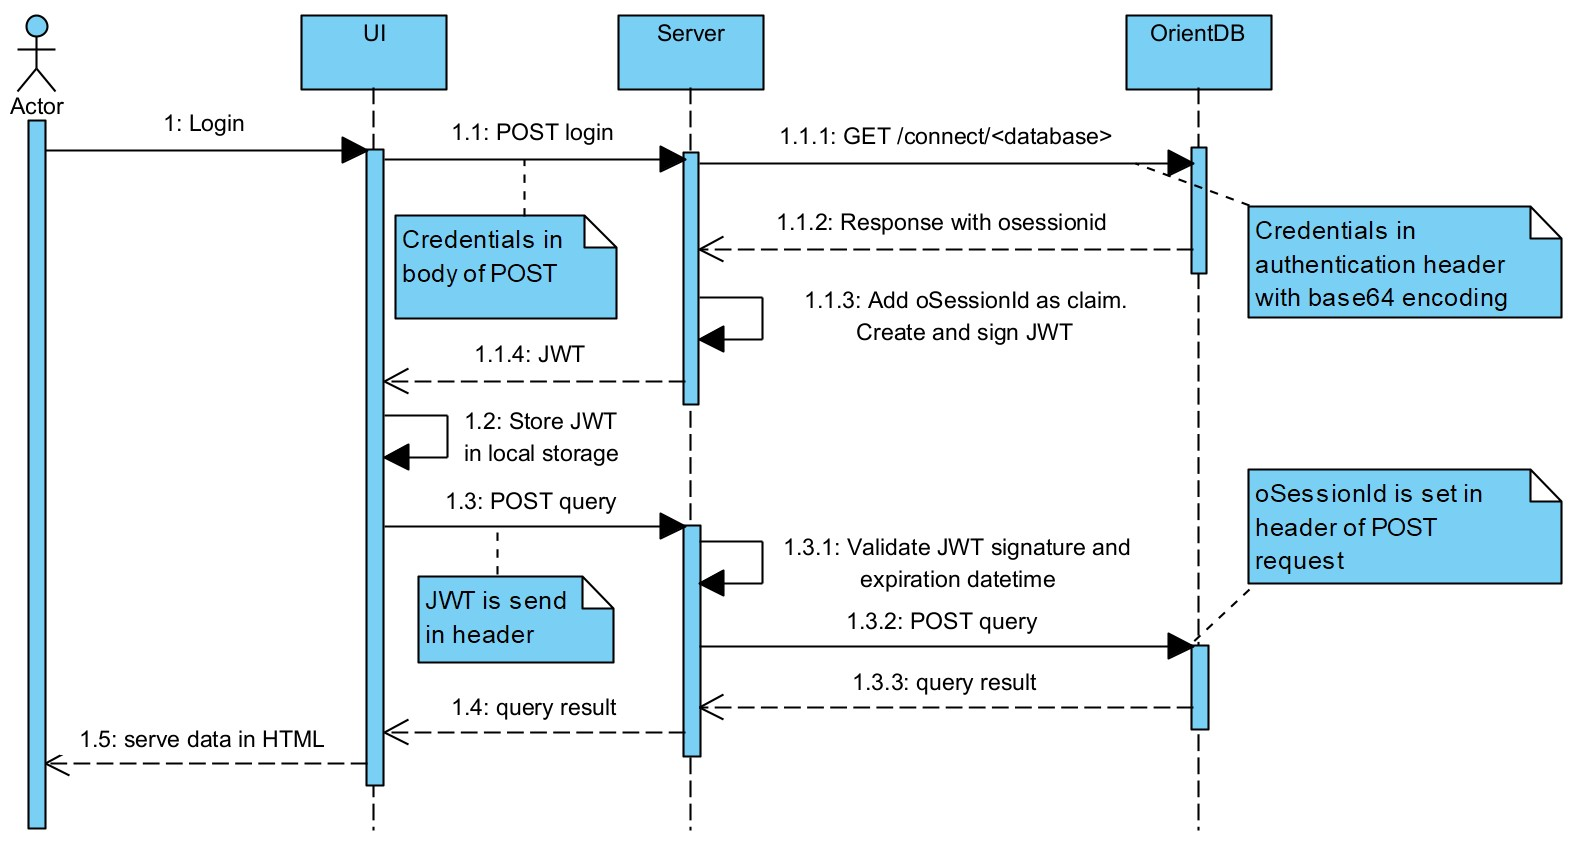
\includegraphics[scale=0.4]{images/authentication-sd.png}
\captionof{figure}{Authentication sequence (UML 2.0)}\label{fig:auth-sd}
\endgroup

An example of the JWT generated by the .NET server is displayed in listing \ref{code:jwt}. The JWT can be decoded by anyone, for example, with a website like \url{https://jwt.io}. The corresponding header and payload are displayed in listing \ref{code:jwt-payload}. In the JWT, two dots are visible, showing the three sections of the token. The first section is dedicated to the header information (lines 1-4 in listing \ref{code:jwt-payload}). The middle section contains the payload (lines 5-12 in listing \ref{code:jwt-payload}). The third and last section contains the signing information, validating the token. 

\begin{lstlisting}[language=xml, caption=Example JSON Web Token (line breaks for display purposes only), style=nonrstyle, label=code:jwt]
eyJhbGciOiJIUzI1NiIsInR5cCI6IkpXVCJ9.eyJodHRwOi8v
c2NoZW1hcy54bWxzb2FwLm9yZy93cy8yMDA1LzA1L2lkZW50a
XR5L2NsYWltcy9uYW1lIjoidGVzdGFyIiwiT3JpZW50RGJTZX
NzaW9uIjoiT1NFU1NJT05JRD1PUzE2NDk3OTY5OTgxODgtMTE
3NTE5OTcxMDIyNDcxNTA0MyIsIkRhdGFiYXNlTmFtZSI6InRl
c3RhcjIiLCJleHAiOjE2NDk4MDA1OTgsImlzcyI6Imh0dHA6L
y9sb2NhbGhvc3QiLCJhdWQiOiJodHRwOi8vbG9jYWxob3N0In
0.zkSDTOuNrn9lR0ca6JLQsbSiLEskEBC_uY937q9sSU0
\end{lstlisting}

The Server signs the JWT (see the self message 1.1.3 in figure \ref{fig:auth-sd}) with a secret provided during the startup of the .NET Server. When the .NET server receives the JWT during a call, it will validate the JWT to ensure it is legit and the information in the payload is not altered.  

There are a couple of interesting claims visible when viewing the payload. Line \verb|6| shows the username of the user. Line \verb|7| shows the OrientDbSession which the .NET server is using to communicate to the graph database. Line \verb|8| displayed the databasename. The databasename is only visible when on the Server the feature 'MultipleDatabases' is activated. Lines \verb|9| (exp), \verb|10| (iss) and \verb|11| (aud) are showing the claims registered in the \acrfull{iana} \cite{jones2015json}. \verb|exp| Stands for 'expiration' and shows the expiration time in seconds (in Unix epoch). By default the expiration time set to 5 minutes, which is the same as the orientdb session id. 

\begin{lstlisting}[language=xml, caption=Decoded JWT header and Payload of the JWT given in listing \ref{code:jwt}, label=code:jwt-payload]
{
  "alg": "HS256",
  "typ": "JWT"
}
{
  "http://schemas.xmlsoap.org/ws/2005/05/identity/claims/name": "testar",
  "OrientDbSession": "OSESSIONID=OS1649796998188-1175199710224715043",
  "DatabaseName": "testar2",
  "exp": 1649800598,
  "iss": "http://localhost",
  "aud": "http://localhost"
}
\end{lstlisting}

\subsection{Hosting the components}
The two new components presented in this thesis, .NET server and the \testar analysis website, need to be hosted on two individual web servers. The .NET server needs to be able to execute server-side code. 

The new \testar Analysis website needs to be hosted on a web server that can host static files. Blazor is interactive by nature, but from a server's perspective, is it a static site since it does not have any server-side code execution. All code executions are handled on the user's computer. Before the user can use the website, it is downloaded on its computer before it gets executed. After the download, the application runs on the user's computer and the traffic to and from the .NET server will not travel through the public internet but stays on the local area network. 

The new \testar analysis website is publicly available on \url{https://app.testarin.net} (read as app dot \testar in dot net). The .NET server needs to be hosted on the network of the user. It needs to be able to access the OrientDB Server. 

To help setting up the two components, two separate docker images are created. Both are available on the docker hub: \verb|rneeft/testar-net-server|\footnote{\url{https://hub.docker.com/repository/docker/rneeft/testar-net-server}} and \verb|rneeft/testar-net-ui|\footnote{\url{https://hub.docker.com/repository/docker/rneeft/testar-net-ui}}.
\section{\ref{rq:what-is-change-detection} What is change-detection, and what do we want to use it for?}

\todo{This should move to related work}


toool made by F-secure. collaboration with Pekka GUI Driver. both had features. 

automated masking abstract away know a lot. image comparison. 

GUITAR, something. 

F-secure change detection point it own 
new tool, no paper. 

Change what we are intresing in.

starting state depends on existng data. external changes removed. 

percent of change pixel could indicate .... div > 50\% change then different. 
1 level-> differences on the screen.
2 level-> change in the model (state graph)
3 level-> Form testing, from testing correct and incorrect form
 - hint faker library phone number etc...
 - relationship between 

find values on the new page. releation input value and one of the screen. you input phonenumber. on screen is presented on

metaphorfic testing (relationships). 

Alexander Pretengkro finding state machine. (Aho can connect).

Anomoli detection for change. most change happen on one stap. What if the it stop changes Trent, history change some... change on change detection. 
 
 source: meeting 2 dec with IVVES 
\section{\ref{rq:useful-detection} Which properties make a model useful for change detection?}

Dynamic are not usable since they can change without detectable reason. \cite{mulders2022Statemodel}
\section{\ref{rq:testar-config} Which \testar configuration will generate a useful model?}
\section{\ref{rq:finding-changes} How can we find changes between two models?} \label{sec:finding-changes}

\todo{This section must have an introduction}

Finding changes is handled in the \verb|Testar.ChangeDetection.Core.Algorithm| namespace. The new analysis website handles the visualisation of the differences and is discussed in section \ref{rq:type-visualisation-answer}. The classes used for the algorithm are visualised in figure \ref{fig:class-diagram-differences}. 

\begingroup
\captionsetup{type=figure}
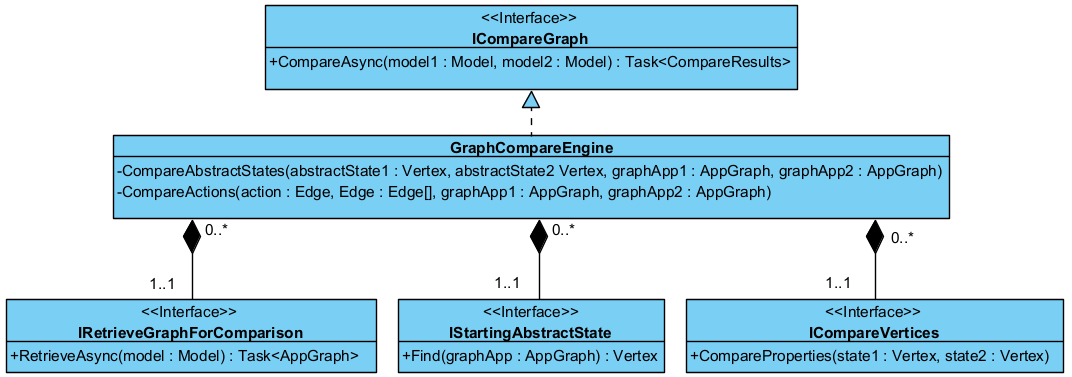
\includegraphics[scale=0.65]{images/4-UML-Differences.png}
\captionof{figure}{Class diagram, algorithm namespace (UML 2.0)}\label{fig:class-diagram-differences}
\endgroup

\subsection{The change detection algorithm} \label{sec:change-detection-algorithm}
The algorithm will be explained in this sub-section, starting with a high-level overview. After the high-level overview, the different interfaces in figure \ref{fig:class-diagram-differences} are explained in more detail.

The concept of \textit{corresponding states} needs to be explained to understand the algorithm. Corresponding states mean that two states, in the new and the old model, are identified as the 'same' state but can have different data. There are a couple of ways to identify corresponding states. The first is by assumption, the second is inferred, and the last is by asking a third party (for example, a human input). For the developed algorithm, only the first two are used. 

Figure \ref{fig:compare-algorithm-start} gives an overview of the start of the algorithm. The \verb|GraphCompareEngine| starts with retrieving the graph data for the old and the new model. This step is indicated by step 1.1. Step 1.2 follows identical actions as 1.1 and is therefore omitted from the diagram.
\newpage

\begingroup
\captionsetup{type=figure}
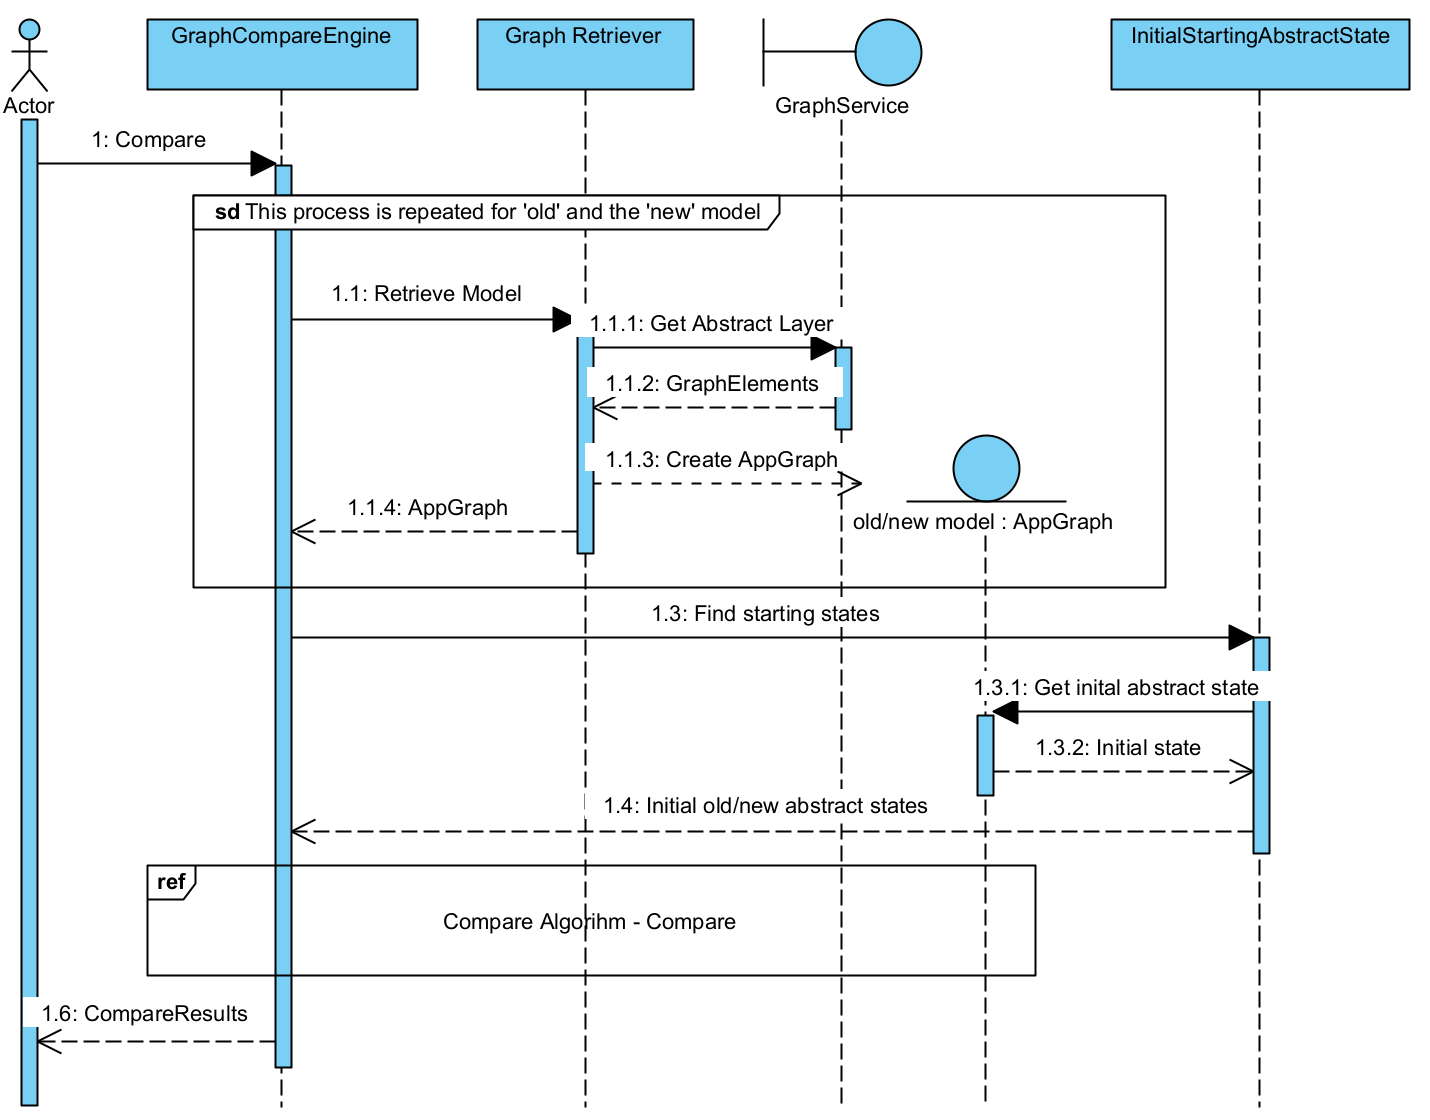
\includegraphics[scale=0.9]{content/5-Results/Images/Compare-algorithm-start.png}
\captionof{figure}{Compare Algorithm (1) - Start (UML 2.0)}\label{fig:compare-algorithm-start}
\endgroup

The next step is finding the starting states, indicated by step 1.3. Those will be the first corresponding states. The current version of the algorithm assumes that the initial states from both graphs are corresponding states. Those states could, for example, be a splash screen or a loading screen.

The flow of the algorithm continues in figure \ref{fig:compare-algorithm-compare} with 1.5. in which the initial states are marked as corresponding states (Step 1.5.1). The rest of the progress follows a recursive pattern between two algorithm methods, the first being \verb|CompareAbstractStates| (Step 1.5) and \verb|CompareActions| (Step 1.5.5).

The algorithm uses the abstract model to find high-level changes within the system under tests. As discussed in section \ref{abstract-model}, the concrete model contains all the information about states within the application under test, and the abstract model contains the abstracted data. Concrete states are abstracted into abstract states, and concrete actions are abstracted into abstract actions. As so, an abstract state contains one or more abstract actions, leading to another abstract state.
 
In step 1.5, the corresponding states are compared. The first step is setting the \verb|IsHandeld| variable to ensure that states are not compared twice. Then the element data of the two abstract states are compared. The comparison is done by the \verb|ICompareVertices| interface and is discussed in more detail on the sub subsection on page \pageref{sec:i-compare-vertices}.

The last step of the \verb|CompareAbstractStates| step enumerates the new model's abstract actions. For each action, the method \verb|CompareActions| (step 1.5.5) is executed, marking the action of the new model as handled. Then it looks in the corresponding abstract state for action with the same \verb|actionId|. The action id is a hashed subset of properties, as was discussed in section \ref{state-identifiers}. 

If an abstract action is found with the same \verb|actionId|, it retrieves both actions' target state. When both states are not handled, it will call the \verb|CompareAbstractStates| (Step 1.5) to make the recursive call. Both states are marked as corresponding states. Finding corresponding states by walking through the action is the second approach to finding corresponding states: inferring.

The code for the change detection algorithm is handheld by four interfaces. Each interface is discussed in more detail below, starting with the \verb|IRetrieveGraphForComparison| interface, which downloads the graph for comparison. Secondly, the \verb|IStartingAbstractState|, responsible for finding the starting states for the comparison, then the \verb|ICompareVertices| interface, which compares the element data for two given vertexes. The last interface is \verb|ICompareGraph|, which will execute the algorithm and depend on the discussed interfaces. 

In the coming sections, the various interface and associated default implementations are explained in more detail.

\textit{Note: When comparing the methods and return values presented in this thesis and the source code, one can find a discrepancy. Some return values are decorated with the} \verb|Task<..>| \textit{object and some method have the suffix} \verb|Async|. \textit{Those technical details are omitted from the thesis since they do not provide any additional value to the algorithm. When a method returns in C\#, it is an asynchronous method that can be awaited by the called. The} \verb|await| \textit{keyword will create a non-blocking call that enabled multi-threading applications \cite{asynchronous-programming}.}

\newpage

\begingroup
\captionsetup{type=figure}
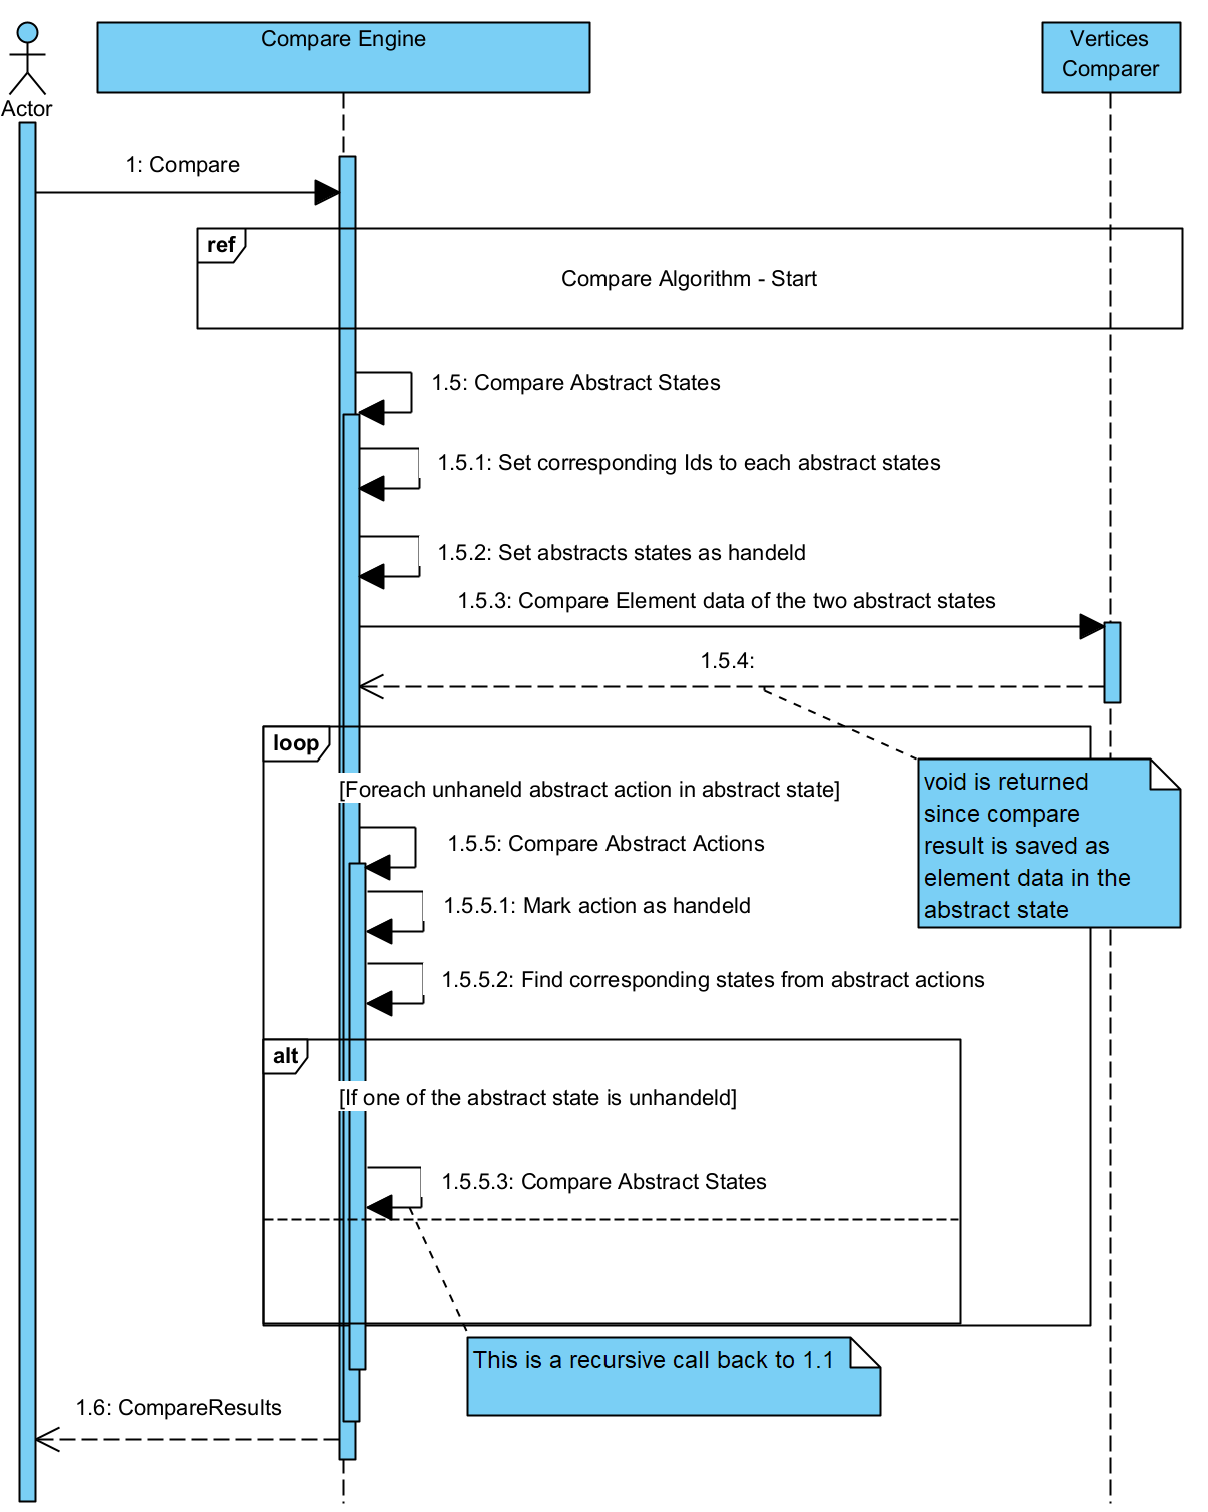
\includegraphics[scale=0.9]{content/5-Results/Images/Compare-algorithm-compare.png}
\captionof{figure}{Compare Algorithm (2) - Compare (UML 2.0)}\label{fig:compare-algorithm-compare}
\endgroup

\subsubsection{IRetrieveGraphForComparison}
The \verb|IRetrieveGraphForComparison| interface is implemented by the \verb|GraphForCompareRetriever| and is responsible for retrieving the graph data from the server. It has a dependency on the GraphService (\ref{sec:the-graph-service}). 

Given a \verb|Model|, which contains the application name and version, the data from the abstract Layer, the concrete Layer and the abstract concrete connectors are retrieved. Only the data from the abstract layer is used for the comparison. The data from the concrete layer and the abstract concrete connectors are downloaded so that they can be used in the visualisation of the presentation of the graph (Discussed in more detail in \ref{rq:type-visualisation-answer}), likewise is the enrichment of the abstract actions with the description from the corresponding concrete actions.

\begingroup
\captionsetup{type=figure}
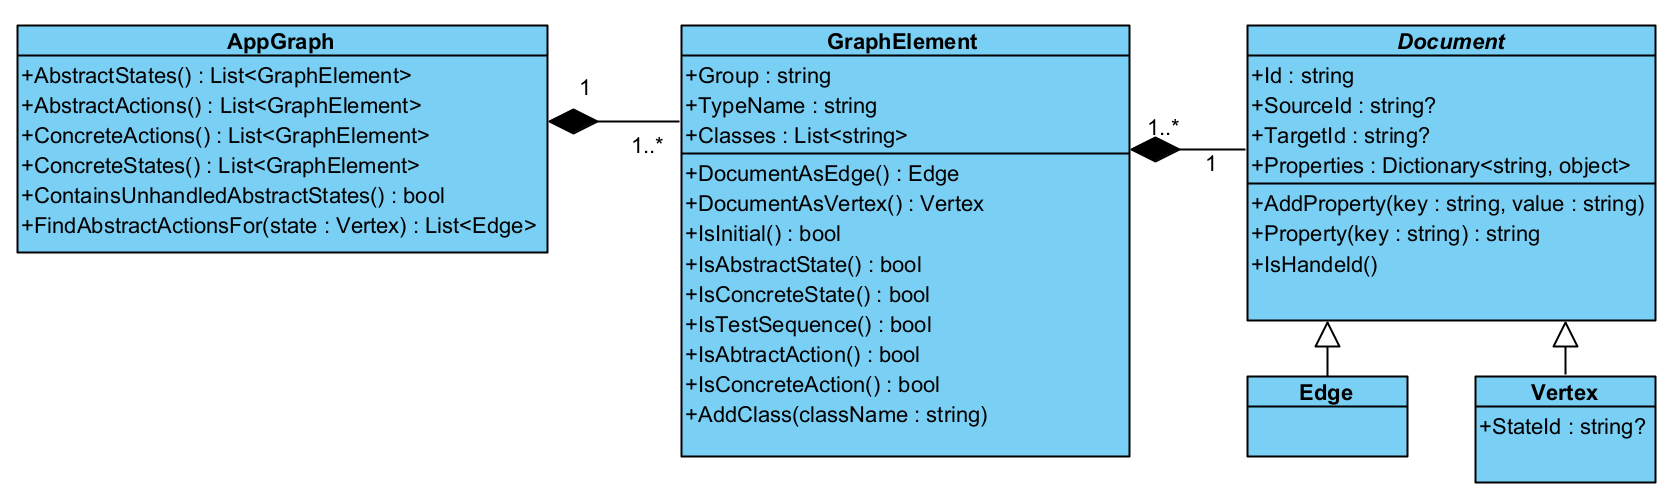
\includegraphics[scale=0.6]{images/4-UML-Models.png}
\captionof{figure}{Class diagram Graph models (UML 2.0)}\label{fig:class-diagram-models}
\endgroup

The \verb|AppGraph| class, shown in figure \ref{fig:class-diagram-models}, is wrapper around a collection of \verb|GraphElement|'s. The \verb|GraphElement| is container a abstract Document which is either a Vertex or an Edge. The abstract \verb|Document| class contains the properties from the vertex or the Edge.

%When the \verb|AppGraph| is serialised into JSON, it will generate the structure that can be read by the Cytoscape Graph visualisation library.

Although the data for each element is located as set of properties, the classes in figure \ref{fig:class-diagram-models} contains some helper properties, e.g. \verb|IsAbstractAction| and \verb|IsConcreteState| which returns a Boolean depending on the type name. 

\subsubsection{IStartingAbstractState} \label{sec:starting-abstract-state}
The interface \verb|IStartingAbstractState| is used to locate at which abstract state the algorithm must start comparing. The default implementation is given by the \verb|InitialStartingAbstractState|. As the class name suggests, this implementation is looking for the initial state. For the correct working of the algorithm, it is assumed that the initial states are corresponding states. For example, the initial states can be a splash or a loading screen.

\subsubsection{ICompareVertices} \label{sec:i-compare-vertices}
When the algorithm finds corresponding states, it needs to compare the states together. This comparison is handled by the \verb|ICompareVertices| interface. A default implementation is provided by the \verb|CompareVertices| class. In algorithm \ref{alg:comparison-corresponding-states} is explained how the inner workings of the implementation are working.  

\begin{algorithm}
    \caption{Vertex comparison}\label{alg:comparison-corresponding-states}
    \begin{algorithmic}
        \Require Element data of old model
        \Require Element data of new model
        \State $O$ = Element data of old model
        \State $N$ = Element data of new model
        \For{$p \in$ $(O \cup N)$}
            \State Mark $p$ as \textit{Added} in new model
        \EndFor
        \For{$p \in$ $(N \cup O)$}
            \State Mark $p$ as \textit{Removed} in old model
        \EndFor
        \For{$p \in$ $(O \cap N)$}
            \State $O_v$ = value of element data in old model
            \State $N_v$ = value of element data in new model
            \If{$O_v \neq N_v$}
               \State Mark element data as changed 
            \EndIf
        \EndFor
    \end{algorithmic}
\end{algorithm}

All the findings of algorithm \ref{alg:comparison-corresponding-states} are saved as element data with the prefix \verb|CD_| (for Change Detection) so that the visualisation can find them easily. Moreover, changed element data is prefixed with \verb|CD_CO_| or \verb|CD_CN_| (respectively CO standing for Changed Old value and CN for Changed New value), and new data elements are prefixed with \verb|CD_A_| (A for added) and removed data elements are prefixed with \verb|CD_R_| (R for removed).

\subsubsection{ICompareGraph} \label{sec:compare-algorithm}
At the start of this section (\ref{sec:change-detection-algorithm}) an high level overview is given concerning the change detection algorithm. The algorithm is implemented by in the \verb|GraphCompareEngine| class and is using the above mentioned inteffaces as dependencies. The \verb|Compare| method is given 

A limitation of change detection is that the object, in this case, the old and new version of an application, needs to be similar enough to enable the detection of changes in the first place \cite{andrews2009visual}. To verify whether the requirement of similarity is met, the used abstract attributes of the two versions are compared, and when different abstract attributes are used, the comparison process is cancelled \cite{stateDiff}. 

%Abstract Graph comparison
%First the software create a ComparableGraph. A Comparable graph only contacts the nodes and edges from the abstract states and abstract actions. The data however will include data from the concrete states and actions. 

%When we have a changed abstract state, get a widget tree of one concrete state
%https://www.xmlunit.org/  have a package for both java as .NET to create differences between version.

%using a fast mode
%the fast mode will only look into changes on the abstract level. Changes like different colours for example


% Every element has an ID generated by OrientDb e.g. #154:0. When merging elements those Id's are merged to by the following algorithm: \#Id1\_Id2 e.g. \#150:0\_\#150:1. 

%difference engine
%merge graph \cite{andrews2009visual}
%the graph needs to be similar are "enough"

%Finding matching notes is done by the difference algorithm. 


\section{\ref{rq:type-visualisation} How to visualise change?} \label{rq:type-visualisation-answer}
In section \ref{sec:finding-changes} the detection of changes between two version of the same application is explained. It showed that having two models the abstract states were compared to find corresponding states. The corresponding states were compared to discover the changes in element data. In this setion the change detection results is used as input for visualising the changes. 

In this section the visualisation of the change detection results are discussed. First the technology is discussed how to show a graph and what is needed for that (section \ref{sec:graph-visualisation}). In section \ref{sec:merge-graph} is explained how the results are used to merge the two graphs and to visualise one single graph.

\subsection{How are graphs visualised} \label{sec:graph-visualisation}

The visualisation of graphs in the new analysis tool is being drawn by Cytoscape.js\footnote{https://js.cytoscape.org/}. "Cytoscape.js is an open-source graph theory (a.k.a. network) library written in JS [JavaScript]" \cite{cytoscape-js}. The cytoscape.js library was used by the build in analysis website of \testar made by Mulder \cite{thesisMulders} and was migrated to the new Analysis website. The Java code that was used to convert the data from OrientDb to a Cytoscape.js acceptable format has been refactored and moved to the new C\# code.

All the information about a model and graph is stored in OrientDB. The new Analysis website is retrieving the model and graph data through the \testar .NET server from the OrientDB database. This communication is done by the \verb|GraphEngine|. The \verb|GraphEngine| contains a method for each layer it, for example: \verb|FetchAbstractLayerAsync|. Edges between layers are retrieved with a different method, for example: \verb|FetchAbstractConcreteConnectors| which retrieves the edges between a abstract and concrete state. By splitting up the method for each layer it becomes possible to only retrieve the information that is needed. As an example, the graph shown for an application, like in figure \ref{fig:graph-page}, needs to have all the information while the detection algorithm only needs the abstract information. 

The \verb|GraphEngine| is retrieving the data from each layer and transforms them into a internal model. A UML class diagram of the internal model can be viewed in figure \ref{fig:class-diagram-models} (the \verb|AppGraph| does not play a role in the displaying the graph). When the transformation from the OrientDB database to graph elements is completed the engine returns them in a list structure. 

Beside the vertexes and edges, the \verb|GraphEngine| can also include a compound object. A compound object grouped graphs objects together. Figure \ref{fig:compound-example} shows such a compound layer which groups the concrete states together into a 'ConcreteLayer'. The new Analysis website has an options, in the settings page, to enable the grouping of items into a compound layer.

\begingroup
\captionsetup{type=figure}
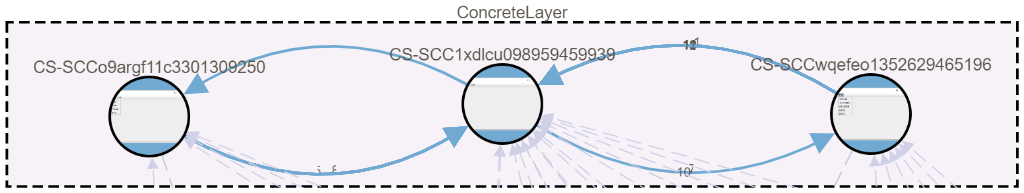
\includegraphics[scale=0.6]{content/5-Results/Images/compound-layer.png}
\captionof{figure}{Compound object grouping concrete states together}\label{fig:compound-example}
\endgroup

After the list with \verb|GraphElement|'s is retrieved, it needs to be passed to the Cytoscape.js library in the form of JSON objects. Since the \verb|GraphElement| is created with the idea of JSON in mind, the serialisation to JSON is easy. An example of the serialisation result can be viewed in listing \ref{code:graph-json}. The data contains an array of elements each having three attributes: \verb|group|, \verb|data| and \verb|classes|. The group is either contains the value nodes or edges, representing their graph element. The attribute \verb|data| contains the \verb|id| of the element and all the additional data about the vertex/edge. For an edge that data also contains the target and source id, specifying the id of a vertex. The element classes is similar as classes in \textsc{CSS} and can be used to style the elements in the GUI. 

\begin{lstlisting}[language=xml, caption=Graph representation in JSON, label=code:graph-json]
[
  {
    "group": "nodes",
    "data": {
      "id": "n100" 
    },
    "classes":[
      "AbstractState"
    ]
  },
  {
    "group": "nodes",
    "data": {
      "id": "n101"
    },
    "classes":[
      "AbstractState"
    ]
  },
  {
    "group": "edges",
    "data": {
      "id":"e99",
      "target": "n100",
      "source": "n101"
    },
    "classes" :[
      "AbstractAction"
    ]
  }
]
\end{lstlisting}

The result of listing \ref{code:graph-json} generates the graph visible in figure \ref{fig:graph-example}. The full HTML code is added as appendix \ref{appendix:cytoscape-example}. 

\begingroup
\captionsetup{type=figure}
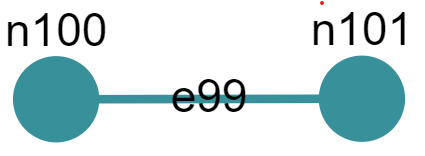
\includegraphics[scale=0.6]{content/5-Results/Images/graph-example.png}
\captionof{figure}{Example graph}\label{fig:graph-example}
\endgroup

\subsection{Merging the two graphs} \label{sec:merge-graph}

After the two models are compared by the change detection algorithm (section \ref{sec:change-detection-algorithm}) a graph can be created which contains both models and the changed detection results. The technique presented by Andrews et al. is used to merge two graphs into one merge graph. Andrews et al. describes an six steps approach in merging two graphs. The algorithm of merging will be explained below in the same six steps.

\subsubsection{1. Read Two input Graphs}

The two models and therefor the two graphs needs to be read. Section \ref{sec:graph-visualisation} explains how the graphs $G_{old}$ and $G_{new}$ are read.

\subsubsection{2. Find Matching Nodes}
This step is handled by the change detection algorithm discussed in section \ref{sec:change-detection-algorithm}.
Results are an enriched version of $G_{old}$ and $G_{new}$. 


\subsubsection{3. Create Merge Graph}
Andrews et al. uses the following algorithm to merge two graphs into a merge graph: "A merge graph $G_m$ is created by combining the two input graphs [$G_{old}$ and $G_{new}$] and considering the matches from $S_m$ [In our case $S_m$ does not exist, instead the corresponding ids between states is used to match nodes in the graph]. First all nodes and edges from $G_{new}$ are added to $G_m$. Then all non-matching nodes from $G_{old}$ are added to $G_m$. Finally all edges from $G_{old}$ are added to $G_m$ and wired, except the edges with the same actionId. Edges which connect to matching nodes from $G_{old}$ have to be connected to the matching nodes from $G_{new}$." \cite{andrews2009visual}. \footnote{Andrews et al. used $G_1$ and $G_2$ to indicate their graphs, the names have been replaced with $G_{old}$ and $G_{new}$}

The edges that were leading to nodes in $G_{old}$ nee to be rewired to nodes in $G_{new}$. To help with the rewiring process two in-memory dictionaries are used. The first dictionary contains the combination of $StateId_{old}$ with $NodeId_{new}$. The second dictionary contains the combinations of $NodeId_{old}$ with $StateId_{old}$. Using the two dictionaries a combination of the following can be made:
\[ NodeId_{old} \rightarrow  StateId_{old} \rightarrow NodeId_{new}. \]
Since the edges contains the Id of both the target and source node, using the two dictionaries the $NodeId_{old}$ can be rewired to $NodeId_{new}$.

\subsubsection{4. Lay Out Merged Graph}

Laying out the merged graph is handled by the Cytoscape.js library as discussed in section \ref{sec:graph-visualisation}.

\subsubsection{5. Propagate Changes to Original Graphs}

The original graphs are not displayed in the compare results. Doing so would take up too much screen space, especially when the graphs can become very big. To provide the options to view the original graphs new classes are added to the merge graph. 

First of all the nodes from $G_{new}$ are given the class 'NewVersion' and if they had a corresponding state the class 'OldVersion', since the matching nodes from $G_{old}$ are not added to the $G_m$. The same is done for all the edges in $G_{new}$. The non-matching nodes and all the edges in $G_{old}$ are given the class 'OldVersion'.

By providing the 'NewVersion' and 'OldVersion' filtering can be applied by Cytoscape.js making it possible to toggle the view into the Old, New and Merge view. 

\subsubsection{6. Manually Edit merged Graph}

This section is not applicable to the New Analysis Website since it does not provide an options to manually set corresponding states in order to change the merged graph. 


\section{\ref{rq:shortest-set} How to generate the shortest set of actions that helps the user to reach the changed state in the SUT?}

\todo{Out of scope?}

\section{\ref{rq:req-apps} What are the requirements for validation applications?}

\todo{Out of scope?}

\section{\ref{rq:validation-apps} Which applications can be used for validation?}

\todo{Out of scope?}